\documentclass[12pt, letterpaper]{article}
\usepackage{graphicx}
\usepackage{hyperref}
\usepackage{xcolor}
\begin{document}
\title{National football victories increase rates of alcohol-related domestic abuse}
\textbf{Letter}:
A Letter is an important research study of high quality and general interest to human behaviour researchers.  The text is approximately 5,000 words, including the introductory paragraph, but excluding references and figure legends. Letters should have no more than 4 display items (figures and/or tables). As a guideline, Letters contain approximately 30 references (excluding those cited exclusively in Methods). This format begins with a title of, at most, 90 characters (including spaces), followed by an introductory paragraph (not abstract) of approximately 200 words, summarizing the background, rationale, main results (introduced by "Here we show" or some equivalent phrase) and implications of the study. This paragraph should be fully referenced and should be considered part of the main text, so that any subsequent introductory material avoids too much redundancy with the introductory paragraph. Letters are not divided by headings, except for the Methods heading.

Letters include received/accepted dates and may be accompanied by supplementary information. Letters are peer reviewed.


\maketitle

\section{Shortintro}

Understanding the potential triggers of violence in family and intimate partner relationships is key for designing effective interventions to protect victims. Previous research (Kirby, Biricombe \& Cafe) has suggested that national football (soccer) tournaments increase rates of reported domestic abuse in England. While hypothesized to be a significant factor, we know little about the role alcohol plays in this relationship. Using crime data from the third largest police force in England from the period 2010-2018, we find that alcohol-related domestic abuse incidents increase by 62\% after an England victory in a national football tournament (World Cup, European Championship). This effect is driven by a 76\% increase in male to female alcohol-related incidents (and is absent from male to male, female to male and female to female domestic abuse incidents), and is not present in other types of criminal behaviours, such as public order offences, other violent, or property-related offences. A three-hour analysis reveals that the increase starts in the three-hour period of the match, the highest in the three hours after the victory, and gradually declines to its baseline level in the 12 hours following the match. \textcolor{red}{Considering repeat incidents that occurred on match days, we did not find that they are characteristically different from other incidents that reoccurred on non-match days.}


\section{Longintro}

"If England gets beaten, so will she" - read the poster as part of the "The Not-So-Beautiful-Game" awareness campaign launched by the National Centre for Domestic Violence in the wake of the 2018 FIFA World Cup. While the link between sporting events and intimate partner abuse has long been in the focus of qualitative sociology (e.g., Sabo et al, 2000), large-scale quantitative investigations of this relationship are relatively scarce. In the US, the most extensive study in the topic was presented by Card \& Lee (2010), who found that an unexpected loss of the local NFL team resulted in a 10\% increase in rates of reported intimate partner violence (IPV).

In the UK, a few studies have investigated the link between football and domestic abuse. Football's history is inextricably linked to England, and is by far the most popular sport in the country, with the World Cup consistently attracting record number of viewers every four years (\textit{citation}). In a small, exploratory study Biricombe and Cafe investigated the effect of the 2010 World Cup on domestic abuse, using data from 33 out of 39 police forces in England. Using a control period from 2009, they found that rates of reported domestic abuse increased significantly when England lost or won (about 33-35\%), but did not change on days then they draw. In a more comprehensive investigation, Kirbey et al used daily counts of intimate partner violence in Lancashire from the 2002, 2006 and 2010 World Cup, and they found a 38\% increase in rates of reported domestic violence when the England team lost, and a 26\% increase when they won or drew. These estimates had been widely discussed in the British media before the 2018 World Cup, and the figures were also quoted on the posters in the Not-so Beautiful Game Campaign.  

However, domestic abuse is unlike most other crimes, and these differences warrant a careful interpretation of these estimates. First, domestic abuse is a vastly underreported crime (the latest figures published by the Crime Survey of England and Wales show that only 17\% of all domestic abuse victims reported the abuse to the police \textit{citation}). Second, domestic abuse should be viewed as a pattern of ongoing behaviour, involving a series of incidents, rather than a one-off incident triggered by football (Brooks-Hay \& Lombard, 2018). These studies, however, still suggest that national football tournaments may create an environment for abusers that is conducive to domestic abuse. While the link between football fandom and domestic abuse is complex...\textcolor{red}{1-2 sentences about hegemonic masculinity in sports - basically presenting the idea that sports fandom can promote an experience of of masculinity where dominance, control and violence is permitted and implicitly encouraged.}



\textcolor{red}{What role might alcohol play in this relationship? Research on alcohol and domestic abuse. It's quite controversial, domestic abusers are more likely to engage in substance abuse, but the pathways are not clear (Peralta et al., 2010). high-rate of co-occurrence, but doesn't appear to be the direct cause (Leonard \& Quigley, 1999), Javaid - "alcohol appears to be a facilitator rather than an instigator of IPV".  Previous quantitative studies havent said much about it. Card \& Lee found that the increase didn't depend on the type of the incident ("no difference in the rise in alcohol-related and non-alcohol related offences"). BUT cultural differences could imply different effects in the UK. Football fandom and alcohol consumption have always been inextricably linked in England ( “win, draw, lose, always on the booze”), and this link is continuously further reinforced by the media (\textit{citation}). Talk about how alcohol involvement can make the abuse more likely without sounding like it can be blamed on the alcohol (insight from qualitative research on how alcohol contributes to it? - 1) abusers use alcohol as a "shield" to excuse their behaviour Javaid, 2015; 2) alcohol may strengthen feelings of hegemonic masculinity, palmer, 2014).} Maybe it would make sense to check if alcohol makes the violence worse?

\textcolor{red}{Hypothesis: maybe we would expect overall DA to go up when E loses (based on previous evidence), whereas andecdotal evidence (NHS spokesperson) suggests increase in drinking when England wins, so we would expect increase in alcohol-related incidents then?}

Here we explore the hypothesis that alcohol plays an instrumental role in the link between national football matches and domestic abuse in England. By comparing the effect of football on domestic abuse with its effect on other types of criminal behaviour, we can assess the extent to which domestic abuse is differs from other crimes. We further explore how the effect differs based on the gender of the perpetrator and the victim, and its temporal dynamics by a three-hour regression. Our data allows us to investigate the history of the domestic abuse incidents that happen on days when England win, and to compare these with other domestic abuse incidents. As a robustness check, we also explore whether the effect is robust to the exclusion of specific years. 

Opinion: \href{https://www.heraldscotland.com/opinion/14432673.football-doesnt-cause-domestic-abuse-men-do/}{Football doesn't cause domestic abuse, men do}.


Opinion: \href{https://www.newstatesman.com/politics/sport/2016/07/what-does-it-mean-when-major-football-tournaments-increase-incidents-domestic}{What does it mean when major football tournaments increase incidents of domestic violence?}.

Drinking \& Football: \href{https://www.independent.co.uk/news/health/world-cup-2018-england-vs-sweden-alcohol-poisoning-hospital-record-number-quarter-semi-final-croatia-a8702961.html}{Record number of people admitted to hospital with alcohol poisoning after England World Cup quarter-final win}.

\subsection{Data description}

To explore these hypotheses, we are using crime data from the West Midlands Police (the third largest police force in England, serving an estimated 2.8 million people in 2017) for the period between 2010 and 2018. Our dataset contains all recorded crimes (with a domestic abuse marker) and specific types of incidents (including domestic abuse incidents). For each record in this dataset, we have information about the time and location of the incident or crime, and the gender and age of the offender and victim. We can also identify repeat offenders and victims by their unique person identifier. Incidents and crimes that are domestic abuse related comprise about 31\% of all recorded crimes and incidents in the dataset. There were three World Cups (2010, 2014, 2018) and two European Championships (2012, 2016) in the period covered by our dataset. 

\href{https://www.gov.uk/government/statistics/police-funding-for-england-and-wales-2015-to-2019}{Police force sizes}.

\href{https://www.nomisweb.co.uk/reports/lmp/la/1967128614/report.aspx#tabrespop}{Population projections}.




\section{Results}

\newpage

\subsection{Where does the increase come from? Male to female, age diff less than 15}

\begin{figure}[htb!]
\centering
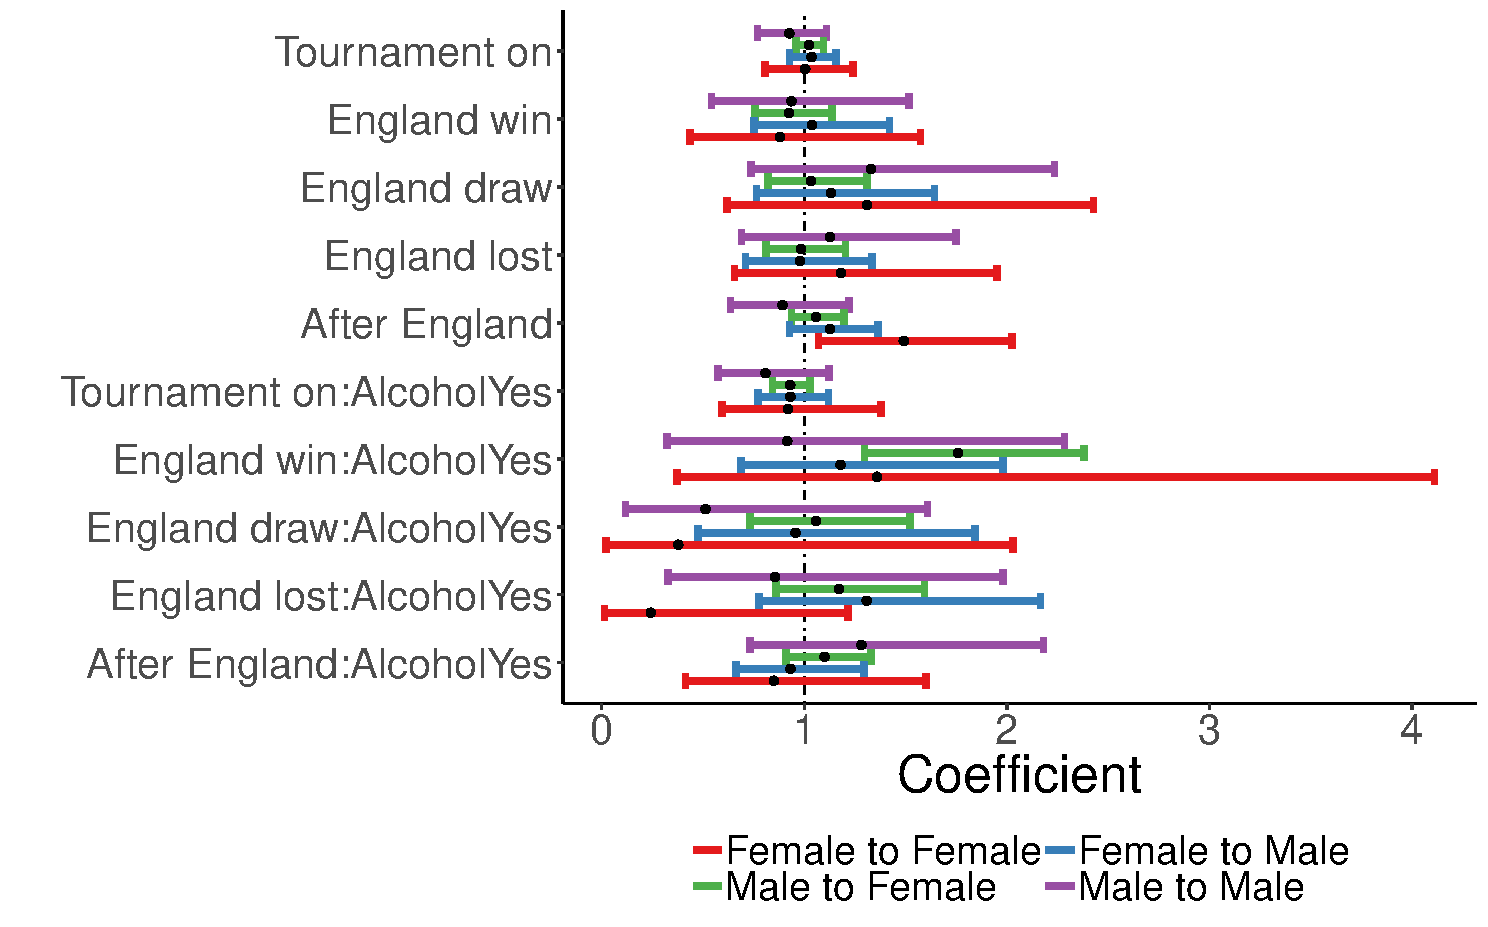
\includegraphics[width=1\textwidth]{DA_gender_compare.pdf}
\label{fig:DA_compare}
\end{figure}

\newpage

\subsection{How does the effect on DA compare to other types of crimes?}


\begin{figure}[htb!]
\centering
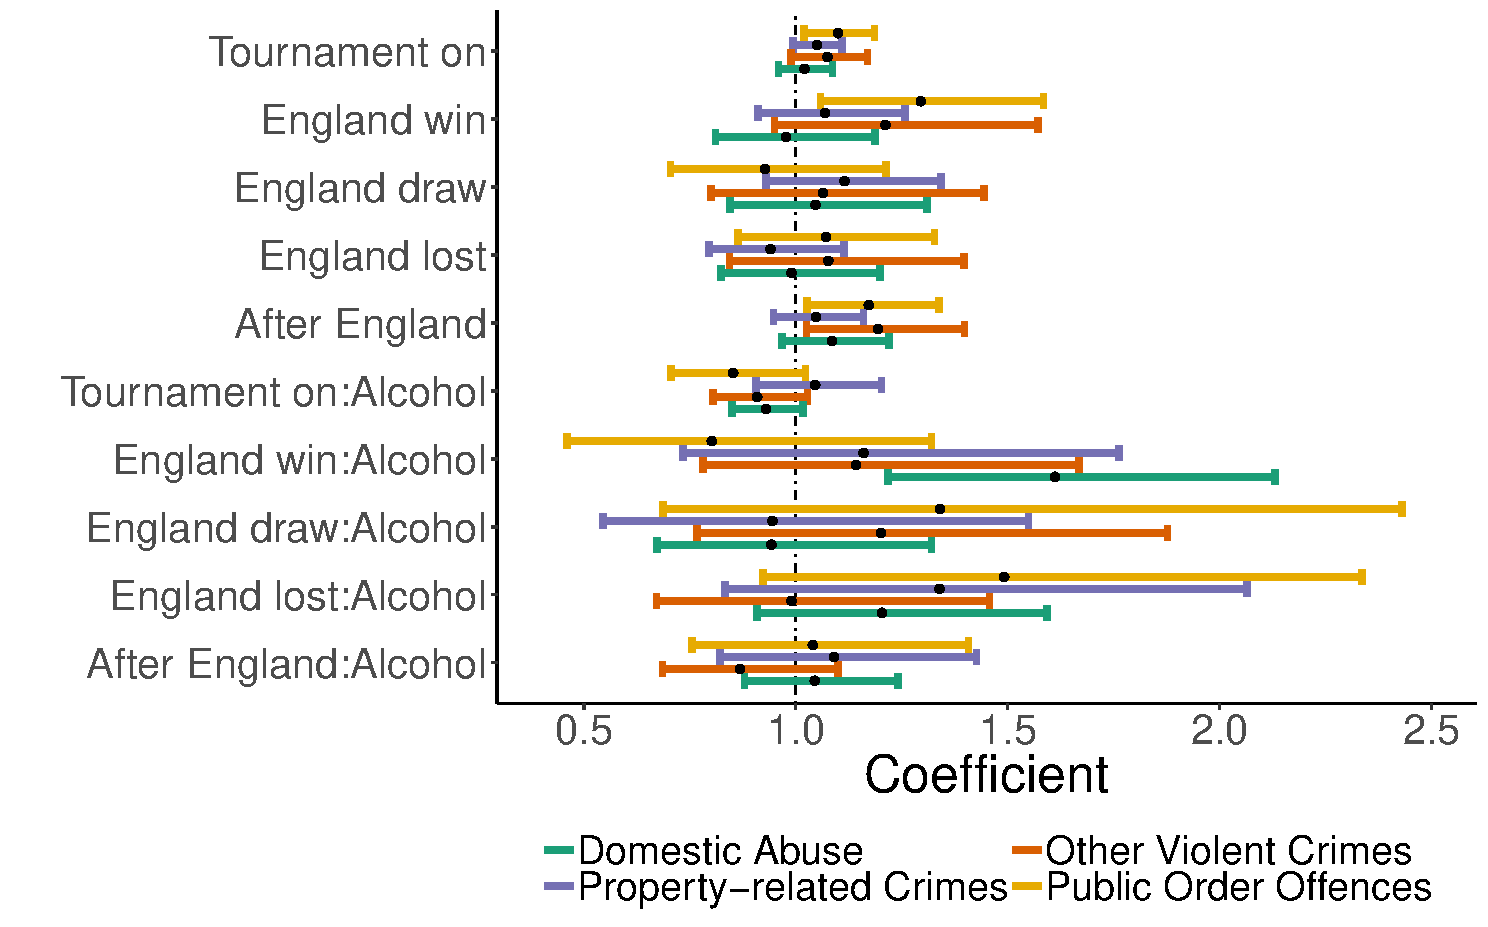
\includegraphics[width=1\textwidth]{DA_compare.pdf}
\label{fig:DA_compare}
\end{figure}

\newpage

\subsection{What can we say about the temporal dynamics of the effect?}
\begin{figure}[htb!]
\centering
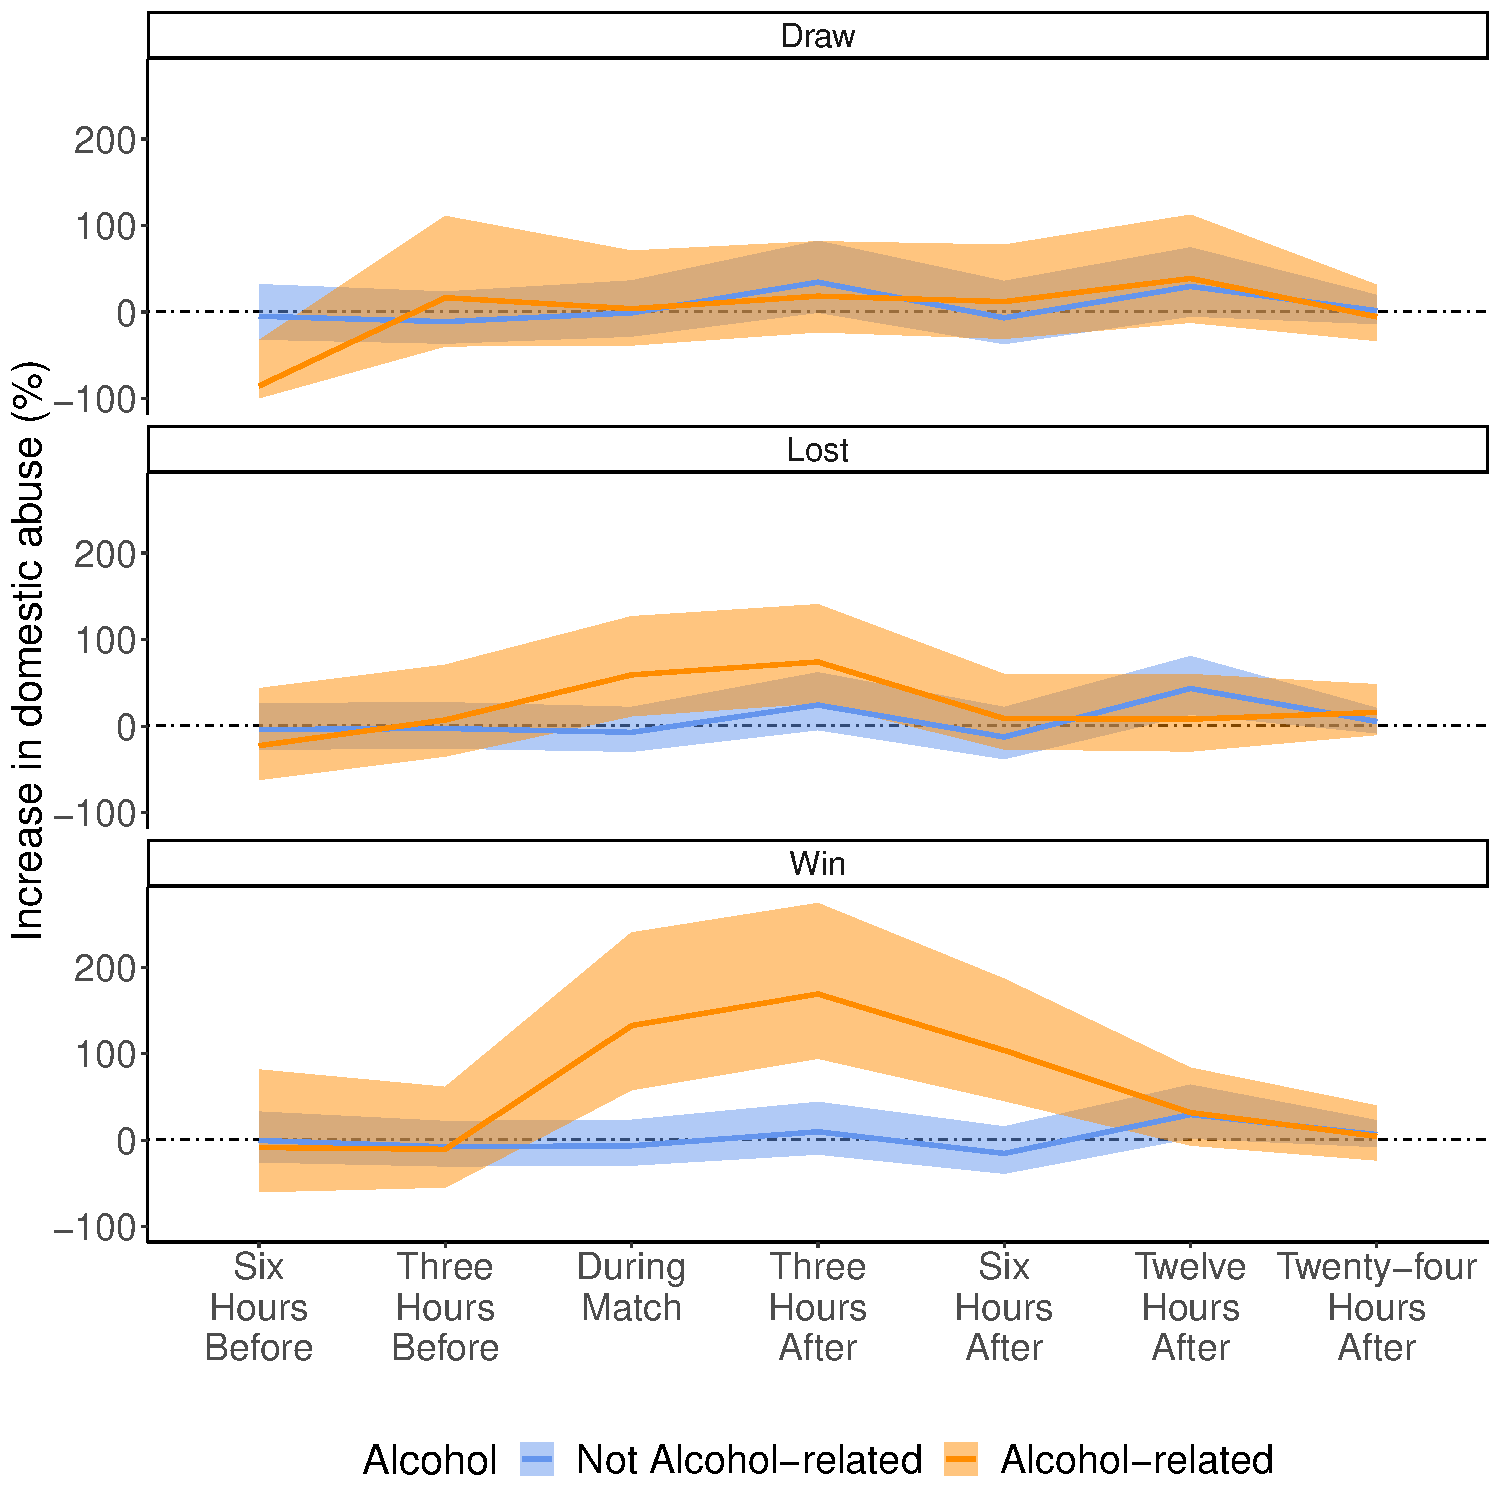
\includegraphics[width=1\textwidth]{Threehours.pdf}
\label{fig:DA_compare}
\end{figure}

\newpage

\subsection{What can we say about repeat incidents that are "triggered" on match days?}




\subsection{Reconciling with previous evidence}

So how can our results be reconciled with those reported previously? Card \& Lee have found an increase in domestic abuse when there is an unexpected loss, but not when the team wins (double check with Neil). An even more striking difference between our results is that they did not find any differential effect on alcohol-related incidents, whereas in our data, the effect is clearly only present in alcohol-related domestic abuse incidents. This discrepancy highlights that the effect on sports-induced emotional cues on domestic abuse are highly sensitive to the cultural context.

As expected, our findings are somewhat easier to reconcile with the results of other, England-based studies. Biricombe and Cafe found an approximately equal increase in domestic abuse when England lost or won, and no increase when they draw. In line with this, our results suggest that there is no increase when England draws - possibly due to the fact that only group-stage, relatively unimportant matches can result in a draw - but we also found an asymmetric effect of losses and wins. Kirby also reported an asymmetric effect, with a 38\% [15 - 66] and 26\% [13 - 40] increase when England lost or win or draw, respectively. However, upon re-analysing their data with separate coefficients for win and draw, and adding a month control, the effects change slightly, indicating a 46\% [29 - 65] increase when England wins, and a 33\% [10 - 59] increase when they lose, respectively, and no effect when they draw. This is more in line with our results, which suggest that while both losses and wins increase rates of domestic abuse, wins have a slightly more pronounced effect. Our results suggests that this asymmetric effect might be down to a large increase in alcohol-related incidents caused by an England victory.




\subsection{Limitations}
underreporting, other factors like weather, campaigns may have increased willingness to report? issues about defining initimate partner violence, maybe increase because people celebrate outside? no.
If he had enough data, we could test for the same thing Card \& Lee have done.

\section{Conclusion}

context - increase in alcohol-related incidents when E wins is 62\%, NYE - 37\%, XMAS - 76\%, Friday - 28\%, Saturday - 102\%, Sunday - 94\%



Why do men abuse women?


Why are men more likely to abuse their female intimate partner after watching sport [REFS? or begin of second para]?

We use a dataset of X,000,000 incidents and crimes in one of England's largest police forces, matched to dates of the three World Cups and two Eurothingies between 20XX and 20XX.

We find a 60 increase in alcohol-related domestic abuse when England wins a world cup or Euro match. 

This effect is large, larger than the  than the effect of a Saturday (48\%)

[This is a large effect, as large as ... sentence about how the effect compares to Christmas, or the effect of a weekday]

The increase reduces to baseline in the three hour period after the game.

The abuse increase does not depend upon whether the abuse is in or away from the home.

We find the increase does not generalise to non-alcohol related domestic abuse and does not generalise to male-on-male or female-on-male, or female on female domestic abuse abuse. 

The effect is not seen for public order offenses, other violent crimes, and property related crimes.  

Football is not the trigger which precipitates abuse with would otherwise occur later. 

Football-related abuse occurs just as soon as other non-football abuse. 

The football related incidents are just as likely to be new incidents of abuse as are non-football incidents. 


Whether the previous incident is alcohol involved is irrelavant.

Theoretical theme :

toxic masculinity, pressure cooker, does alcohol CAUSE abuse, football changes reporting not actual abuse.

Together, this suggests Football-related abuse is just like other abuse. 


Figure 1.

OVerall abuse by football and alcohol to get 60 illustrated

Figure 2. Breakdown by sex pairs and age-gap to show its male-on-female intimate partner

Figure 3. Football-alcohol increase and crime type. It's just domestic abuse.

Figure 4. Timing (a) Three hour plot, and (b) maybe time to previous and next event.

Paragaph 2 is on previous football-domestic abuse research.

Paragraphs on why men abuse women, one on reporting bias, one on alcohol comorbid or causal

\end{document}
